\chapter{Background Notions}
\label{cha:background}

\section{NDP101 Architecture Overview}
\label{sec:architecture}
This is a MCU developed by Syntiant\cite{description_ndp101}, which is a company specialized in Edge AI device development. NDP stands of Neural Decision Processor and is an architecture specialized in deep learning algorithm with audio processing application, like keyword speech interface, sensor applications and speaker identification. The device is composed by two parts, the TinyBoard, which contains the CPU that handles the peripherals, being the hardware part, and a Syntiant NDP101 Core, in which happens all the audio processing and where the Neural Network is stored in. It is important to notice that the DNN (Dense Neural Network) Architecture is fixed, dedicating to 256KB with int32 bias length and int4 weights, which can be at most 589.000, with a total memory. The neural network for this device to be fast enough in computation avoid the use of CNN (Convolutional Neural Network), but can only support 4 Fully Connected Layers, 3 intermediate with 256 neurons and one for output with at most 64 output classes, with classification. To perform the internal software computation there is an internal SRAM inside the chip which is a Cortex-M0 112KB size. This piece of memory contains the binary user's code alongside the global and local variables.
\begin{figure}[!h]
    \centering
        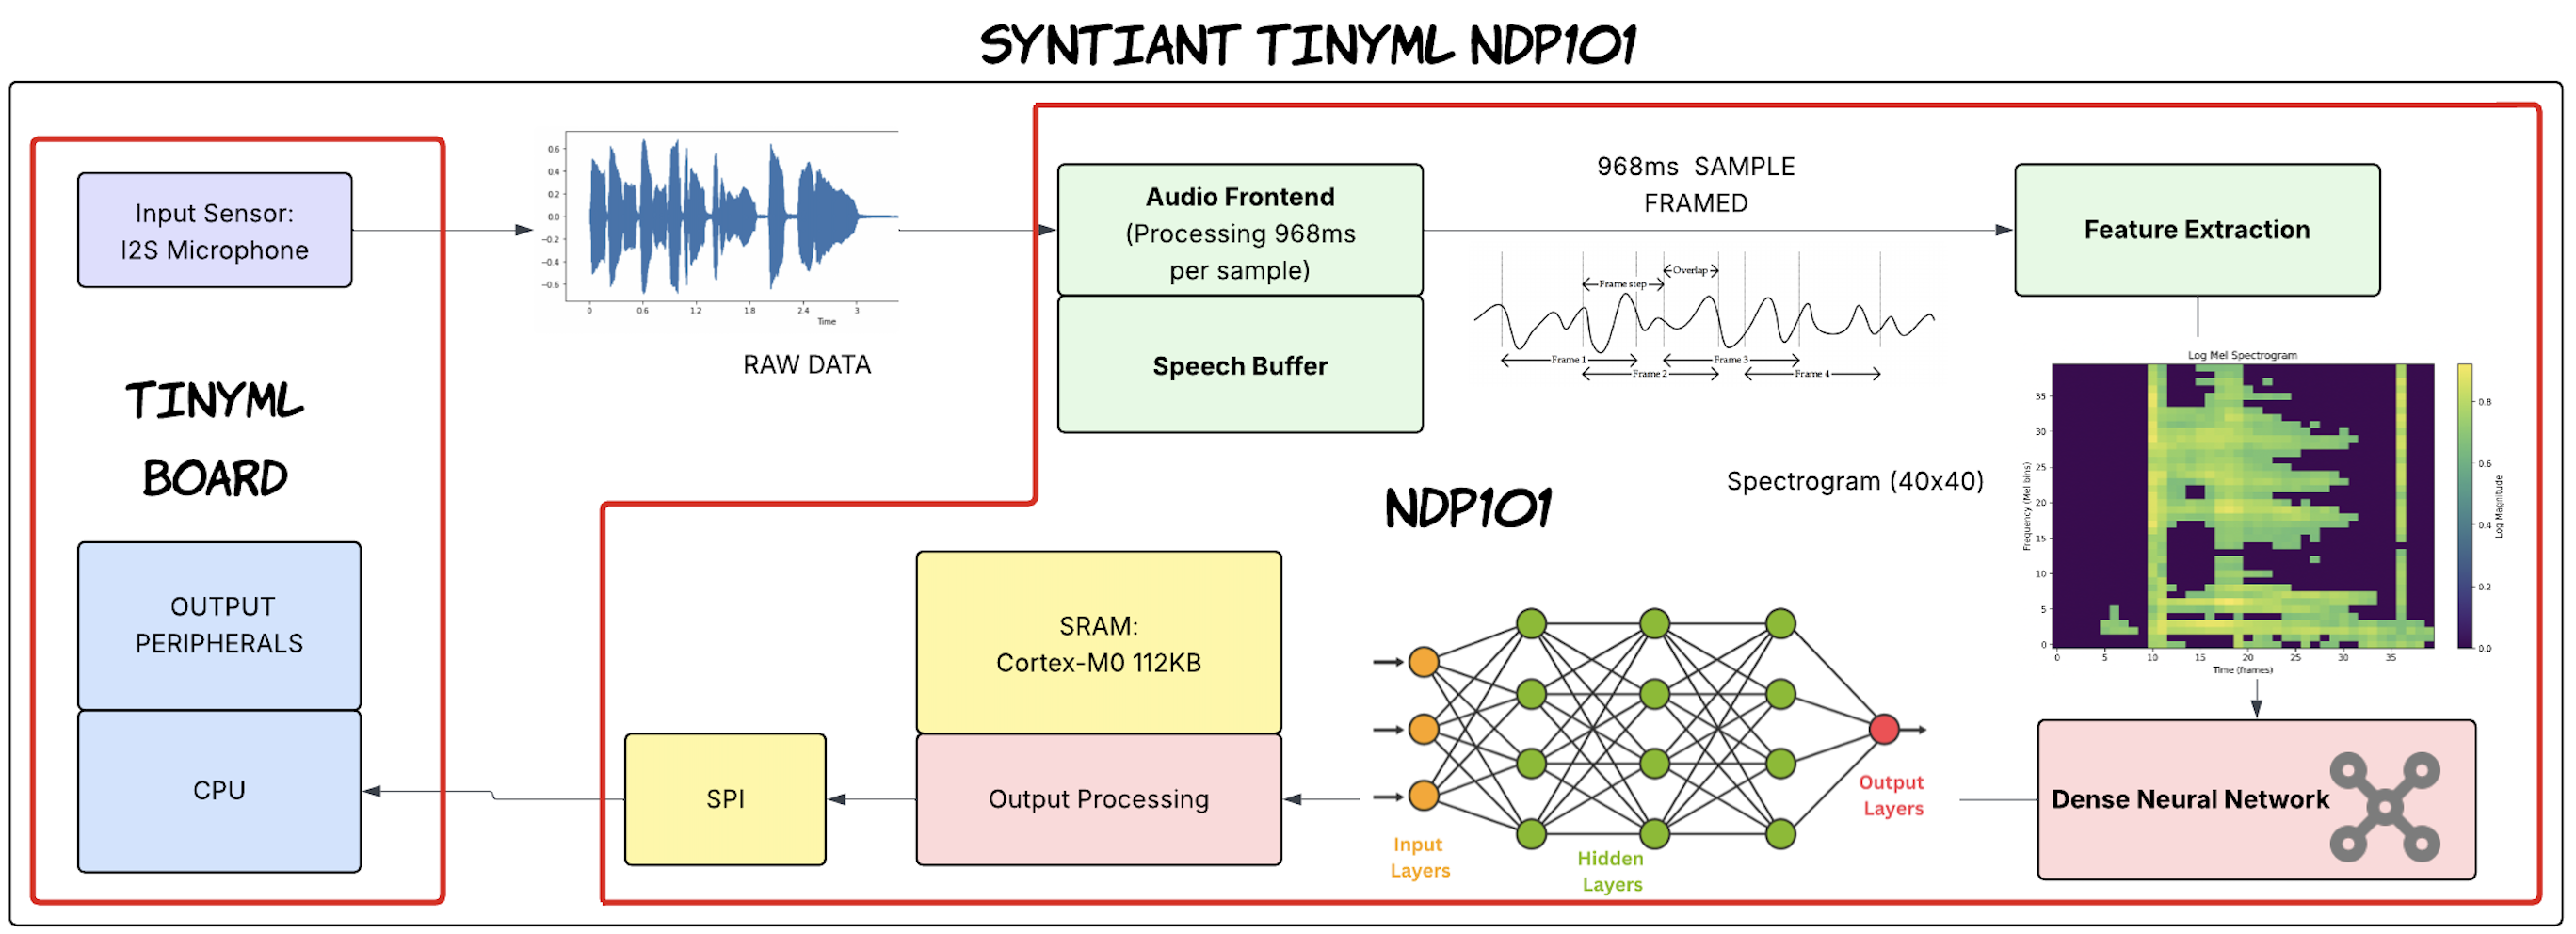
\includegraphics[width=0.9\textwidth]{images/2.01 NDP101 High Level Workflow.png}
        \caption{Syntiant NDP101 High Level Workflow}
\end{figure}
\newline A typical behavior of the device is the following. Starting with a I2S microphone input sensor, which if active will be always on, performing a polling behavior. The input is processed by the Audio Front End, which will perform samples of 968ms, in the meanwhile the system feeds a 96KB speech buffer. These samples are gave in input to the feature extraction that acts like a MFE Block Processing\cite{syntiant_audio_block}, using log-mel spectrogram. This spectrogram will always have 1600 features which will correspond to a 40x40 Spectrogram image. This image is processed by the Dense Neural Network. As default Syntiant NDP101 performs classification, but how the output is used is up to the programmer that can write a code to manage the output of the neural network using Arduino IDE. 
The peripherals of the device, other than the microphone are 9 pins, 4 for power supplying and 5 for GPIO (General Purpose I/O). Other than the Serial Flash Memory (SRAM), there is a micro-SD card slot used for memory extension. In this thesis, we will not use it but for big data storage and for the IMU functionality, supported by the device, that is required and is estimated that with a 32GB card it will save more than 3 days of uncompressed audio data, with a frequency of 16kHz and with IMU more than 300 days of 6-axis sensor data with a frequency of 100Hz. As following there is a image of the principle peripherals connections:
\begin{figure}[!h]
    \centering
        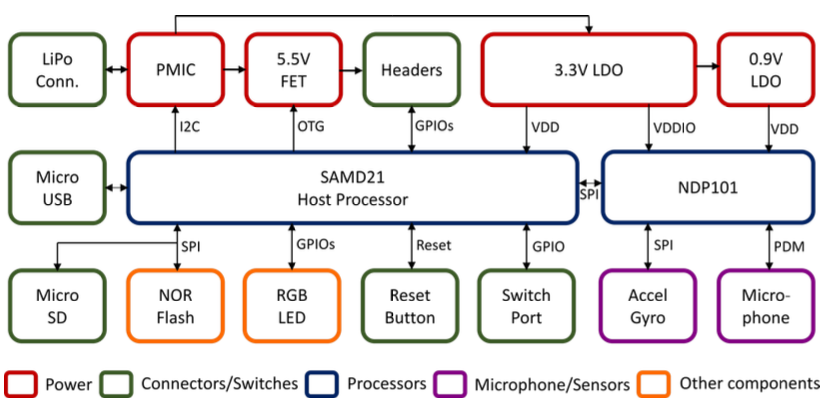
\includegraphics[width=0.9\textwidth]{images/2.02 Design with peripherals.png}
        \caption{Design NDP101 with peripherals}
\end{figure}
\newpage
Power metrics taking \cite{analysis_syntiant_performances}, considering that NDP101 is an always-on power consumption application it manages to use for audio/voice recognition applications 140$\mu$W and these results compared to other CPU will deliver 20 times more throughput and 200 times less energy per inference. The connection with another MCU is possible with SPI communication, however without the SDK provided is Syntiant, is difficult to program setup up it.
%\begin{wrapfigure}{l}{0.5\textwidth}
%  \begin{center}
%    \includegraphics[width=0.48\textwidth]{images/2.03 TinyML Board Structure.png}
%  \end{center}
%  \caption{Syntiant NDP101 External Structure}
%\end{wrapfigure}
\section{Syntiant Audio Block Processing}
\label{sec:audio}
Edge Impulse reports that Syntiant Audio Block Processing is similar to MFE one\cite{syntiant_audio_block}. This block objective is to process the raw data input in a input source extracting time and frequency features from this signal and in Syntiant case deffers a little because of a noise floor at the end of the computation. The block, which corresponds to the feature extractor, can be viewed as following:
\begin{figure}[!h]
    \centering
    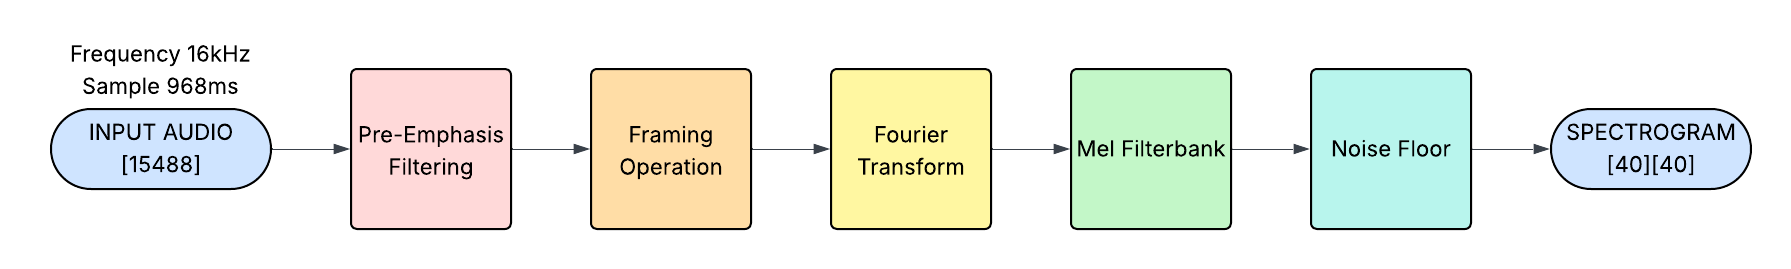
\includegraphics[width=1.0\textwidth]{images/2.03 MFE Block Processing.png}
    \caption{Syntiant Audio Block Processing}
\end{figure} 
1. Input - The frequency of raw data input is at 16kHz and sampling 968ms, it corresponds in having 15488 raw data, with short values vecause the audio sound can go from -$2^15$ to $2^15-1$. These values come from an implicit ADC (Analog Digital Conversion), because Syntiant NDP101 has a dual PDM microphone input which interfaces with I2S interface multiplexed with PDM\cite{PDM_module}. It stands for Pulse Density Modulation and it reduce the system into a single-bit digital one. This allows signal processing operations to be performed on the audio stream easily and then the PDM can be modified by the system in  \newline
2. Pre-emphasis filter - This is a high-pass filter that enhances high-frequency components, so the microphone will capture more low-frequency noise and increase high frequencies to make the speech clear. Before this is needed a audio normalization [-1, 1], generating floats values and then apply this high-filter:
\begin{equation}
    y[n]=x[n]-\alpha\cdot x[n-1]
\end{equation}
$\alpha$ consists in a coefficient of filter grade and a standard Syntaint Block set it at 0.96875\newline
3. Framing - This audio is split and segmentate into small window called frames. Each frame has an overlap time with each other and in Syntiant corresponds to 128 floats, considering the size of 512 floats and the stride, how much the start position will move of 384. In the last frame a part will overflow the initial buffer and in that case the void values are flatted to 0. Considering the input of 15488 samples in a 16kHz frequency:\newline
\begin{equation}
    number\,of\,frames=\frac{input\,size-frame\,size}{frame\,stride}+1=\frac{15488-512}{384}+1=40
\end{equation}
For each one frame of the forty frames are computed:\newline\newline
3.1 Windowing - Before performing Fourier Transform, it's applied a windowing to reduce spectral leakage in integration. It is used the following sinusoidal function in each frame:\newline
\begin{equation}
    0.54-0.46\cdot(\frac{2\pi k}{size-1})
\end{equation}
The size will be 512 and k is an incremental value that goes from 0 up to 511 and k-window is multiplied to the k-position of the array.
3.2 Fast Fourier Transformation (FTT) - This function computes the complex frequency spectrum of a real-valued signal captured in time-domain. It is not required to compute all the DFT domain, because dealing with real value using Hermitian symmetry property with real values, it is require to compute only $\frac{N}{2}+1$ unique complex outputs. 
\begin{equation}
    \begin{cases} 
        X[k]=\sum_{n=0}^{N-1}x[n]\cdot e^{\frac{-2\pi ikn}{N}} & k=0,1,...,\frac{N}{2}\\
        X[l]=\overline{X[k]} & l=N-k
    \end{cases}
\end{equation}
In this case x[n] is the input signal with n=0,...,N-1, x[n]$\in\mathbb{R}$, i is the imaginary unit, k is the incremental value and N is the length of the signal (512 values).
3.3 Spectrogram Population - Corresponds to a magnitude computation of the FFT output, obtaining the amplitude spectrum from the complex frequency-domain data. This computed the norm of the first half of the fourier transformation output and saves it in the corresponding size [40x256], the magnitude is computed as follows:
\begin{equation}
    |X[k]|=\sqrt{(Re(X[k]))^2+(Im(X[k]))^2},\,\,for\,k=0,1,...,\frac{N}{2}-1
\end{equation} 
4. Mel-filterbank - After obtaining this matrix, the algorithm applies a mel-filterbank, which is a set of data based on human perception system via a triangular bandpass filter, making the system more sensitive to low frequencies. It is used the mel scale to obtain this phenomenon, because using a logarithmic approach allows a better sound recognition.\newline
Internal in the software system is created a K+2 length filter called m, composed by linear spaced elements, with K the number of filters.
\begin{equation}
    m[i]=M_{min}+i*\frac{M_{max}-M_{min}}{K+1},\,\,i=0,1,...,K-1
\end{equation}
$M_{min}$ and $M_{max}$ corresponds to the conversion in mel-scale of the minimum and the maximum frequency. Syntiant as default has set the minimum to 0 and the maximum to $\frac{f_s}{2}$. After that it reconverts back in the frequency scale. The conversion formulas are for Syntiant:
\begin{equation}
    m=1127\cdot log_{10}(1+\frac{h}{700})\,\,\,\,\,\,h=700\cdot 10^{\frac{m}{1127}}-1
\end{equation}
To, this scale is applied a triangular filter for each filter between 1 and K, using bins covering frequencies. The computation of the bins and of the triangular function is:
\begin{equation}
    b_i=\lfloor \frac{2\cdot f_i}{f_s}\cdot(N-1)\rfloor\,\,\,\,\,H_k[b]=
    \begin{cases}
        0 & b<b_k-1 or b>b_k+1\\
        \frac{b-b_{k-1}}{b_k-b_{k-1}} & b_{k-1}\leq b \leq b_k\\
        \frac{b_{k+1}-b}{b_{k+1}-b_k} & b_k \leq b \leq b_{k+1}
    \end{cases}
\end{equation}
mel filterbank (pre-emphasis, framing, fft, mel scaling), mfe vs mfcc\newline

\section{Deep Learning Overview}

\section{Keyword Spotting Approaches}
\label{sec:kws approaches}
Classification, softmax

\section{Speaker Verification Approaches}
\label{sec:sv approaches}
text-dependent vs independent sv, general methods not suitable for tinyml (gmm-ubm, i-vectors), d-vector concept, tinysv approach \newline

\newpage